\chapter{Analisi del problema}

La progettazione di un simulatore di un sistema ferroviario presenta diverse problematiche relativamente alla concorrenza e alla distribuzione, in quanto:
\begin{itemize}
	\item il problema prevede l'interazione tra una popolazione di entità in maniera concorrente;
	\item vi sono dei punti di sincronizzazione tra le entità, che devono essere identificati e modellati opportunamente;
	\item non è ragionevole fare assunzioni a priori sulle tecnologie che risolveranno il problema, ne sull'ambiente di esecuzione;
	\item è opportuno prevedere un certo livello di distribuzione delle componenti del sistema;
	\item si possono presentare difficoltà nella trasmissione di dati tra le componenti dovute all'inaffidabilità della rete.
\end{itemize} 
Di seguito andrò ad analizzare gli aspetti più problematici, in termini di Concorrenza e Distribuzione.

% ########################################### DISTRIBUZIONE ##################################################
\section{Distribuzione}

Le problematiche legate alla distribuzione sono molteplici. Nel progetto di un simulatore di un sistema ferroviario infatti, la presenza di entità distribuite è auspicabile, sia per suddividere logicamente le entità, sia per distribuire l'onere di calcolo su nodi differenti.
Le caratteristiche desiderabili da un sistema distribuito che simula una struttura ferroviaria sono:
	\begin{itemize}
		\item Il complesso deve apparire all'utente come un sistema unitario, la natura distribuita del sistema deve essere nascosta all'utilizzatore finale. 
		\item L'architettura distribuita non deve limitare le funzionalità desiderate.
		\item \'E desiderabile che vi sia un buon grado di disaccoppiamento tra le componenti, e dalle tecnologie adottate per la comunicazione tra nodi della rete.
		\item Il sistema dovrà essere il più possibile robusto agli errori.
		\item La progettazione architetturale deve prevedere un meccanismo che permetta Avvio del sistema e Terminazione ordinata.
		\item L'architettura distribuita deve sottostare a vincoli temporali propri di un sistema ferroviario.
		\item La struttura distribuita deve essere tale da permettere estendibilità e scalabilità.
	\end{itemize}

	\subsection{Gestione del Tempo}
	
	La simulazione è scandita da orari di partenza e di arrivo dei Treni che circolano tra le stazioni. Per questo è importante dotare il sistema di un \ii{riferimento temporale} adeguato, che permetta di gestire i ritardi introdotti dalla comunicazione di rete, o dalla diversità di sincronizzazione degli orologi dei diversi nodi della rete.
	 
	Tale problema assume forme diverse in base al grado di distribuzione scelto per le componenti che generano gli eventi caratterizzanti la simulazione. In particolare, un livello di distribuzione alto, che prevede ad esempio la collocazione di una entità Stazione per nodo della rete, richiederà un meccanismo di regolazione del tempo più complesso e delicato rispetto ad un sistema con un livello di distribuzione più contenuto, che preveda ad esempio una distribuzione di singole Regioni di simulazione. 
	
	La scelta del riferimento temporale diviene quindi cruciale per lo svolgersi della simulazione. Abbiamo due tipi possibili di orologio:
		\begin{itemize}
			\item Assoluto: Prevede l'esistenza di un'entità dalla quale le varie componenti attingono per ottenere l'informazione temporale. 
			\item Relativo: Ciascun nodo di calcolo possiede un proprio riferimento temporale interno.
		\end{itemize}
		
	\'E chiaro che la prima soluzione non si presta ad essere utilizzata per il problema presentato. Infatti esso, possedendo un flusso continuo interno del tempo, non permetterebbe a entità indipendenti su nodi diversi di eseguire logicamente allo stesso istante (ad esempio due treni che in nodi diversi partono contemporaneamente da una stazione)

	\subsection{Acquisto di un Biglietto}
	
	In base al grado di distribuzione della modellazione realizzata, è necessario prevedere una struttura distribuita di biglietterie, in quanto la natura del problema prevede un livello di conoscenza globale soprattutto per l'acquisto di biglietti di treni a prenotazione.

	\subsection{Terminazione del Sistema}
	
	La durata di una simulazione di un sistema ferroviario è per sua natura indefinita. \'E quindi necessario un intervento esterno che ne decreti la terminazione.	La \ii{Terminazione del sistema} globale deve essere coordinata tra tutte le componenti distribuite, ed effettuata in modo tale da non far terminare l'esecuzione in uno stato inconsistente. Dovrà inoltre garantire che nessun nodo di calcolo rimarrà attivo (ad esempio, nessun thread in esecuzione o in attesa).

	\subsection{Avvio del Sistema}
	
	L'\ii{Avvio del sistema} dove essere progettato in modo tale da permettere a tutte le componenti distribuite di interagire, ed evitare errori. In particolare:
	\begin{itemize}
		\item dev'essere previsto un meccanismo che permetta una rapida individuazione dei nodi con i quali ciascuna entità coopera;
		\item devono essere evitati (o gestiti) errori causati dal tentativo di comunicazione di thread concorrenti con entità non ancora pronte o allocate.
	\end{itemize} 
	


% ########################################### CONCORRENZA ##################################################
\newpage
\section{Concorrenza}

	Nell'analizzare le problematiche di concorrenza, è necessario individuare quali saranno le entità che svolgeranno un ruolo attivo all'interno della simulazione, e quali un ruolo reattivo, in base alle azioni compiute dalle entità attive. 
	Nella simulazione di un sistema ferroviario, ho individuato le seguenti entità attive:
		\begin{itemize}
			\item Treno
			\item Viaggiatore
		\end{itemize}
	mentre le entità reattive principali saranno:
		\begin{itemize}
			\item Segmento
			\item Piattaforma
		\end{itemize}
	
	\subsection{Ingresso in un Segmento da parte di un Treno}\label{ingresso_segmento}

	\begin{figure}[htbp]
		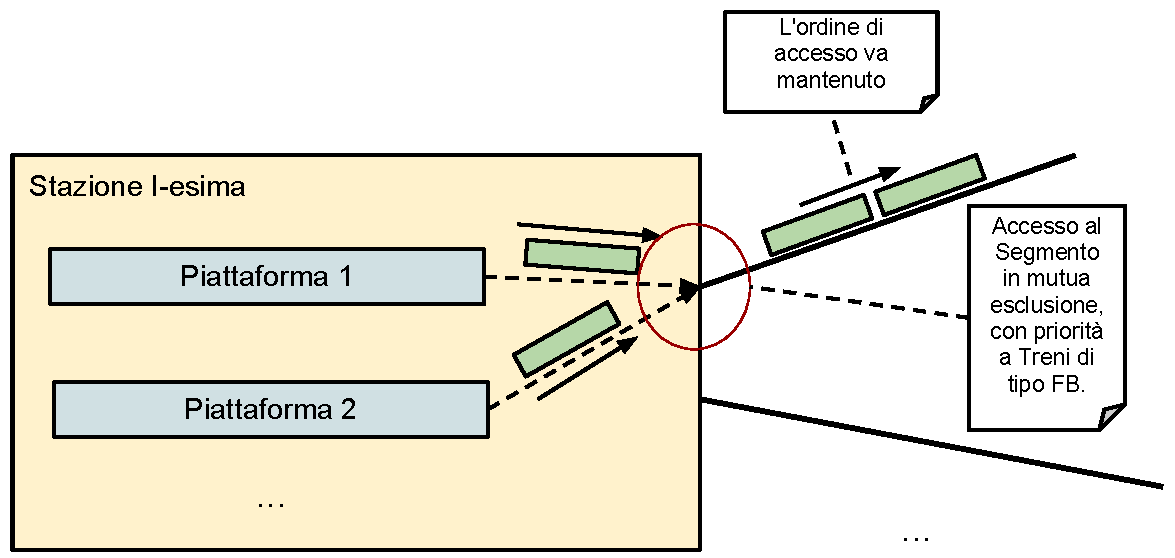
\includegraphics[width=\textwidth,keepaspectratio]{imgs/ingresso_segmento.pdf}
		\caption{\footnotesize{Accesso ad un Segmento da Parte di uno o più Treni.}}
	\end{figure}

	L'accesso ad un segmento di collegamento tra due stazioni da parte di un Treno, è inerentemente concorrente. Tale azione presenta infatti i seguenti requisiti:
		\begin{itemize}
			\item L'ingresso presso un Segmento deve avvenire in \ii{mutua esclusione}; è infatti impossibile che due o più entità Treno accedano ad uno stesso Segmento contemporaneamente.
			\item Più Treni possono circolare su un Segmento contemporaneamente. Questo comporta:
				\begin{itemize}
					\item il mantenimento di un ordine di ingresso al Segmento;
					\item la regolazione della velocità di transito di ciascun Treno in base alla velocità di quelli che lo precedono;
					\item l'impossibilità di un Treno di accedere ad un Segmento qualora vi siano altri Treni che lo percorrono in senso opposto.
				\end{itemize}
			\item Dev'essere data precedenza d'accesso al Segmento, ai Treni di tipo \ttt{FB}.
		\end{itemize}


	\subsection{Uscita da un Segmento e accesso alla Stazione}

	\begin{figure}[htbp]
		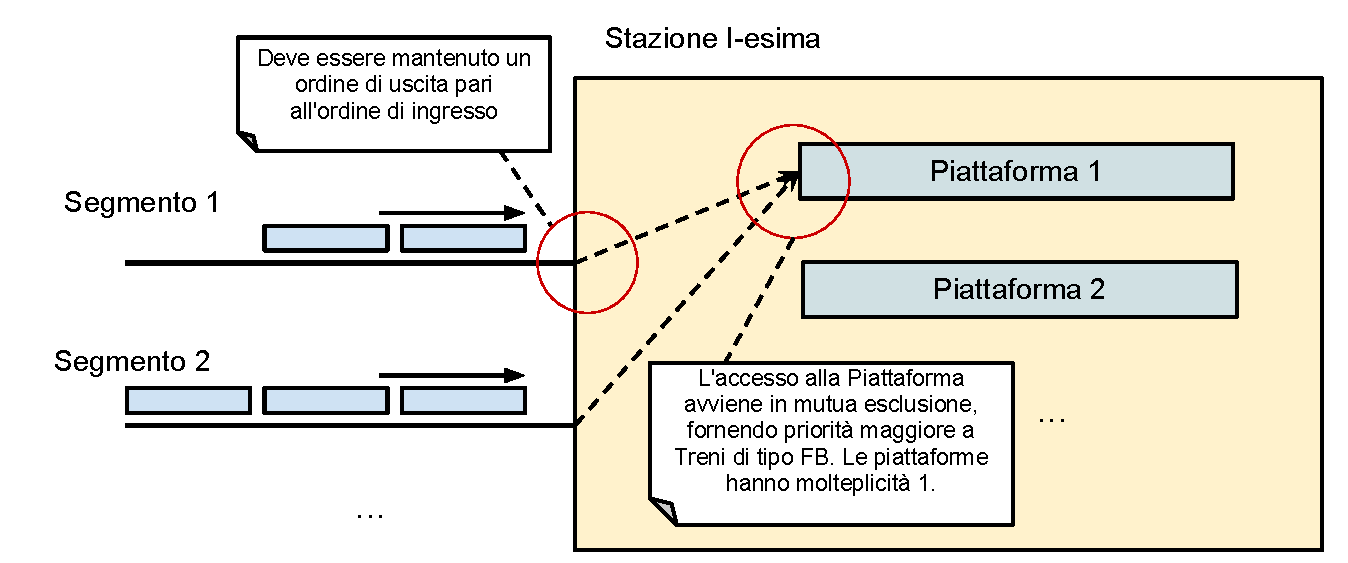
\includegraphics[width=\textwidth,keepaspectratio]{imgs/Ingresso_Stazione.pdf}
		\caption{\footnotesize{Uscita da un Segmento e accesso ad una Piattaforma di uno o più Treni.}}
	\end{figure}

	Il problema introdotto in sezione \ref{ingresso_segmento}, vincola i requisiti che dovranno essere soddisfatti relativamente all'uscita da un Segmento e conseguente accesso alla Stazione successiva. Per quanto riguarda l'uscita dal Segmento avremo quindi i seguenti requisiti:
		\begin{itemize}
			\item L'ordine di ingresso al Segmento dev'essere mantenuto all'uscita. 
			\item L'ordine di uscita da un Segmento dev'essere mantenuto nell'accesso alla stazione successiva da parte dei Treni in transito.
		\end{itemize}

	L'ingresso in una Stazione, permette ad un Treno di occupare una della Piattaforme disponibili e, dato che da specifica una stazione può essere raggiunta da più Segmenti, tale azione sarà svolta in modo concorrente tra i treni in uscita dai vari Segmenti, secondo i seguenti vincoli:
		\begin{itemize}
			\item I Treni di tipo \ttt{FB} avranno priorità maggiore nell'occupare una Piattaforma.
			\item Ciascuna Piattaforma è acceduta in mutua esclusione, e può essere occupata da un solo Treno alla volta.  
		\end{itemize}

	Questo significa che l'accesso ad una Piattaforma sarà ordinato, per tutti i Treni provenienti dallo stesso Segmento, in base all'ordine di uscita da quest'ultimo, e concorrente tra Treni provenienti da Segmenti diversi. 

	\subsection{Acquisto di un Biglietto da parte di un Viaggiatore}

	Ciascun Viaggiatore deve acquistare un biglietto prima di poter usufruire dei servizi ferroviari. Per fare ciò, all'interno ogni stazione vi è una Biglietteria presso la quale l'acquisto può essere effettuato. Un biglietto sarà composto da una serie di Tappe, ciascuna relativa ad un tratto del percorso da portare a termine con uno specifico Treno, sia Regionale che FB. 
	L'assegnazione di un Biglietto ad un Viaggiatore è semplice se il suo percorso prevede solo l'utilizzo di Treni Regionali, mentre è più complesso se vi sono tappe da raggiungere con Treni FB, i cui biglietti vengono erogati se e soltanto se vi è ancora posto all'interno del treno.
	\'E quindi necessario prevedere l'esistenza di una \ii{biglietteria centrale} che mantenga le prenotazioni dei Treni di tipo FB. Si ricavano quindi i seguenti requisiti:
		\begin{itemize}
			\item La biglietteria centrale va acceduta in mutua esclusione, in modo da evitare prenotazioni inconsistenti di Biglietti.
			\item L'erogazione di biglietti può fallire in caso non vi siano posti per percorrere alcune tappe; il sistema deve reagire di conseguenza.
		\end{itemize}

